\section{Experiment's Procedure}


In this chapter, the procedure of the experiment is discussed and thoroughly analysed. We conducted a user study in order to test and analyse our proposed technique, Fat Finger. Each user participating in this study, should follow the instructions given to him, complete the experimental part and finally provide us an assessment. The procedure followed for each participant consist of the following parts. 

\emph{Welcoming - Verbal instructions - Demographic information  - Calibration - Experiment - Assessment}


The elements for each of them will be discussed, interpreted, and visualized with descriptive figures. Duration of each Experiment procedure was calculated to last around 50 minutes. Adding to it the time needed for the instruction and the final assessment we end up having a study that requires about one hour to be fully completed. Apart from that, we should mention that, whilst being an anonymous user study a camera was used to record each participant during the experiment. To keep anonymity, the camera was only focusing on the participants hand and the iPad of course. The basic aim behind using a camera to record each experiment, is that this will very likely make it possible to observe many interesting traits on the way participants use their finger to interact with the UI (User Interface). We might be able to detect different techniques or ways of interaction used among the users. Finally it can be a vital tool on reasoning on weirdly acquired or ambiguous 
collected results.
%%%%%%%%%%%%%%%%%%%%%%%%%%%%%
%%%%%%%%%%%%%%%%%%%%%%%%%%%%%
%%%%%%%%%%%%%%%%%%%%%%%%%%%%%
%%%%%%%%%%%%%%%%%%%%%%%%%%%%%
%%%%%%%%%%%%%%%%%%%%%%%%%%%%%
%%%%%%%%%%%%%%%%%%%%%%%%%%%%%
\subsection{Verbal Instructions}

In the beginning of the experiment a set of instructions (see Appendix \ref{verbalFatFinger}) was given to the participants. Instructions are divided into an introductory and an explanatory part. On the first part, explanatory, the experimenter introduces himself and welcomes the participant. At this point, the participants rights should be explained to the participant. He is allowed to withdraw from the experiment, any time he desires if he feels uncomfortable. Also it is mentioned that this study is anonymous so we will keep no personal information on him. After that we thank him for participating and helping us in this study. Finally we give him a short speech, about the purpose of this study and what we are trying to achieve.

At this point we assign him a \textbf{User Id} and pass him the Demographic information form, which explained in detail in Section \ref{sec:demographic}.

After having filled in the Demographic information form, we are ready to move to the explanatory part. Here, we start by explaining the various aspects we will encounter through this experiment. Firstly the 4 different types of trials are presented and thoroughly explained to him. Before proceeding to the next step we need to make sure that they understood the differences on the targets, the feedback, and also the way of confirming target selection on each type. Then we advise them that they should be as fast and accurate as possible during the trials. Finally, they were advised that in case they fatigue occurs or they just need a break during the experiment, they are welcome to do so, but only when the "Next Trial" button is visible on screen. That way the break will not affect at all the parameters of the experiment.




%%%%%%%%%%%%%%%%%%%%%%%%%%%%%
%%%%%%%%%%%%%%%%%%%%%%%%%%%%%
%%%%%%%%%%%%%%%%%%%%%%%%%%%%%
%%%%%%%%%%%%%%%%%%%%%%%%%%%%%
%%%%%%%%%%%%%%%%%%%%%%%%%%%%%
%%%%%%%%%%%%%%%%%%%%%%%%%%%%%
\subsection{Demographic Information}
\label{sec:demographic}

Demographic Information form is used to collect several basic information about the participant of this study. However, to ensure confidentiality we do not ask them to fill in their  name, surname or address. The fields that need to filled in by the user are:


\begin{itemize}
	\item \textbf{Age}. Age is based on the year of birth, and not on the actual date. 
	\item \textbf{Gender}. Male or Female.
	\item \textbf{Optical Aid}. None, Glasses, or contact lenses. 
	\item \textbf{Handedness}. Right, Left or Ambidextrous.
\end{itemize}

According to these fields we can easily categorize the participants into corresponding groups, and export meaningful results (see Chapter 6).

Finally we ask users to rate their experience in using touch-based mobile devices, and also in using tablet devices. Ranking is based on a 5 point rate scale; very inexperienced (1) to very experienced (5). We also query them if they own, or at least have used a tablet devices and a touch-based device before. In specific:

\begin{itemize}
	\item \textbf{Do you own a tablet device (e.g. iPad)?}

	\emph{Yes - No}
	\item \textbf{Have you used a tablet device before?}
	
	\emph{Yes - No}
	\item \textbf{How do you rate your experience with touch-based mobile device?}

	\emph{Highly inexperienced (1) - Highly experienced (5)}
	\item \textbf{How do you rate your experience with tablet devices?}

	\emph{Highly inexperienced (1) - Highly experienced (5)}
\end{itemize}


The printed version of the Demographic information form can be found in Appendix \ref{demographicFatFinger}, with all the information included. 




%%%%%%%%%%%%%%%%%%%%%%%%%%%%%
%%%%%%%%%%%%%%%%%%%%%%%%%%%%%
%%%%%%%%%%%%%%%%%%%%%%%%%%%%%
%%%%%%%%%%%%%%%%%%%%%%%%%%%%%
%%%%%%%%%%%%%%%%%%%%%%%%%%%%%
%%%%%%%%%%%%%%%%%%%%%%%%%%%%%
\subsection{Calibration}

This section is devoted on the finger calibration process. Calibration is a very important parameter, and necessary too. Since fingers sizes vary among people. The application should be recalibrated for each participant, so as to better match his unique hand dimensions. Thus, it consist an indivisible part of our study, and takes place just before the start of the experiment. When we are calibrating we simply let the system measure the dimensions of our index finger. That way the system will be trained to understand if we are barely, merely or fully touching the screen.

There are many possible ways a user can calibrate his finger, or even better, each finger can be calibrated with more than one ways. Calibration is a very subjective parameter. Each participant is allowed to calibrate his finger the way he feels more comfortable. During the calibration process we simply let the system know which is our desired minimum and maximum contact area size. 


There are two (2)  basic techniques for alternating the contact size of the on-screen covered area.

\begin{itemize}
	\item \textbf{Alternate the \textit{angle} of your finger}. Touch your finger almost vertically to the screen to set the minimum contact area size, and move towards a horizontal position to the set the maximum desired value. Please note that the maximum and minimum values are not the ones that are actually possible. They are the preferred ones. If a user wants to perform smaller movements with hi hand then he may adjusts the values to have a shorter range. However if someone wants to perform longer and bigger movements, they he is welcome to set the minimum and maximum values accordingly.

	\item \textbf{alternate the \textit{pressure} applied}.  Apply no pressure to set the minimum desired contact area and enough pressure the set the maximum desired point. The same rules for the desired and possible values apply here too.
\end{itemize}


However some guidelines were given to them, to help them perform it properly.
\begin{enumerate}
	\item Touch the screen softly with a medium contact size. This movement should be as natural as possible. No need to apply pressure or tension at all.
	\item Move your finger to the desired minimum level. Again there is no need to apply any pressure on the device. The participant should be as relaxed as possible.
	\item Move your finger to the desired maximum level. the allowed part of the finger that can be used as contact area is delimited by first joint point. (Show a figure with that)
	\item From this maximum position please lift your finger. 
\end{enumerate}

After performing those steps, the participant may proceed to the Visualization screen. In this view, he is able to play around with the interface which is calibrated according to the previously acquired input values. ( give a figure). When he fills confident that the calibration is well responding to his finger movement then he may proceed to the experiment. Otherwise, he can calibrate again as many times he wants, until he is completely satisfied with the visualization outcome.

Finally we should also mention that there are two basic techniques users followed for alternating the contact area. In the first we keep all our fingers tight together, and only the index finger is pointing. To change the contact size we need to move our palm and arm. This causes increased fatigue after long term use. On the second one, we simply relax our palm on the table, in a position that only the index finger will be touching the iPad screen. This way alternation of the contact size is effortless and produces the minimum amount of fatigue to the finger.




\begin{figure}[H]
\centering
\begin{subfigure}[b]{0.4\textwidth}
	\centering
	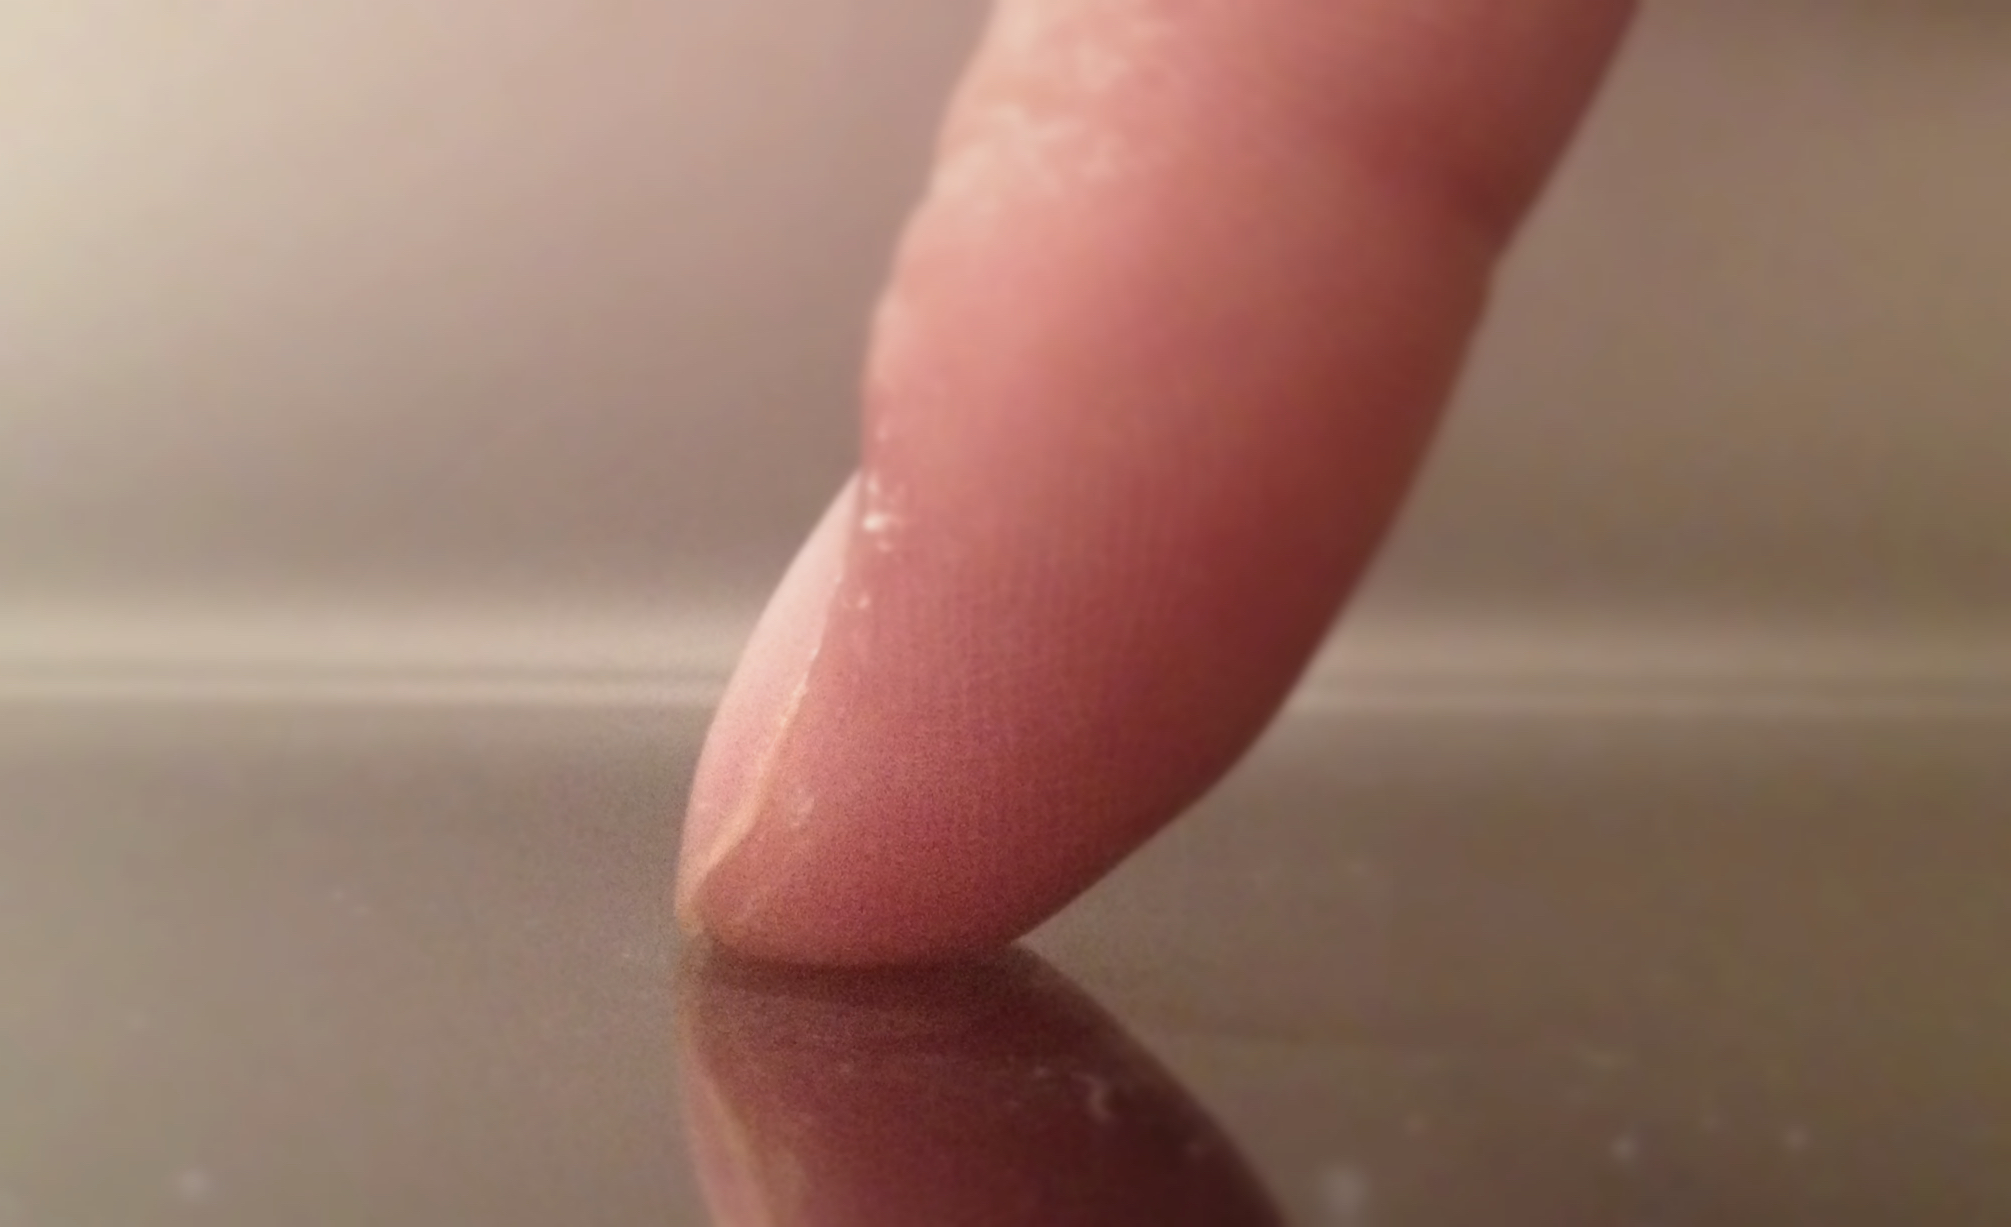
\includegraphics[width=\textwidth]{figures/ffmin}
	\caption{Minimum contact size position}
	\label{fig:ffmin}
\end{subfigure}
\hfill
\begin{subfigure}[b]{0.4\textwidth}
	\centering
	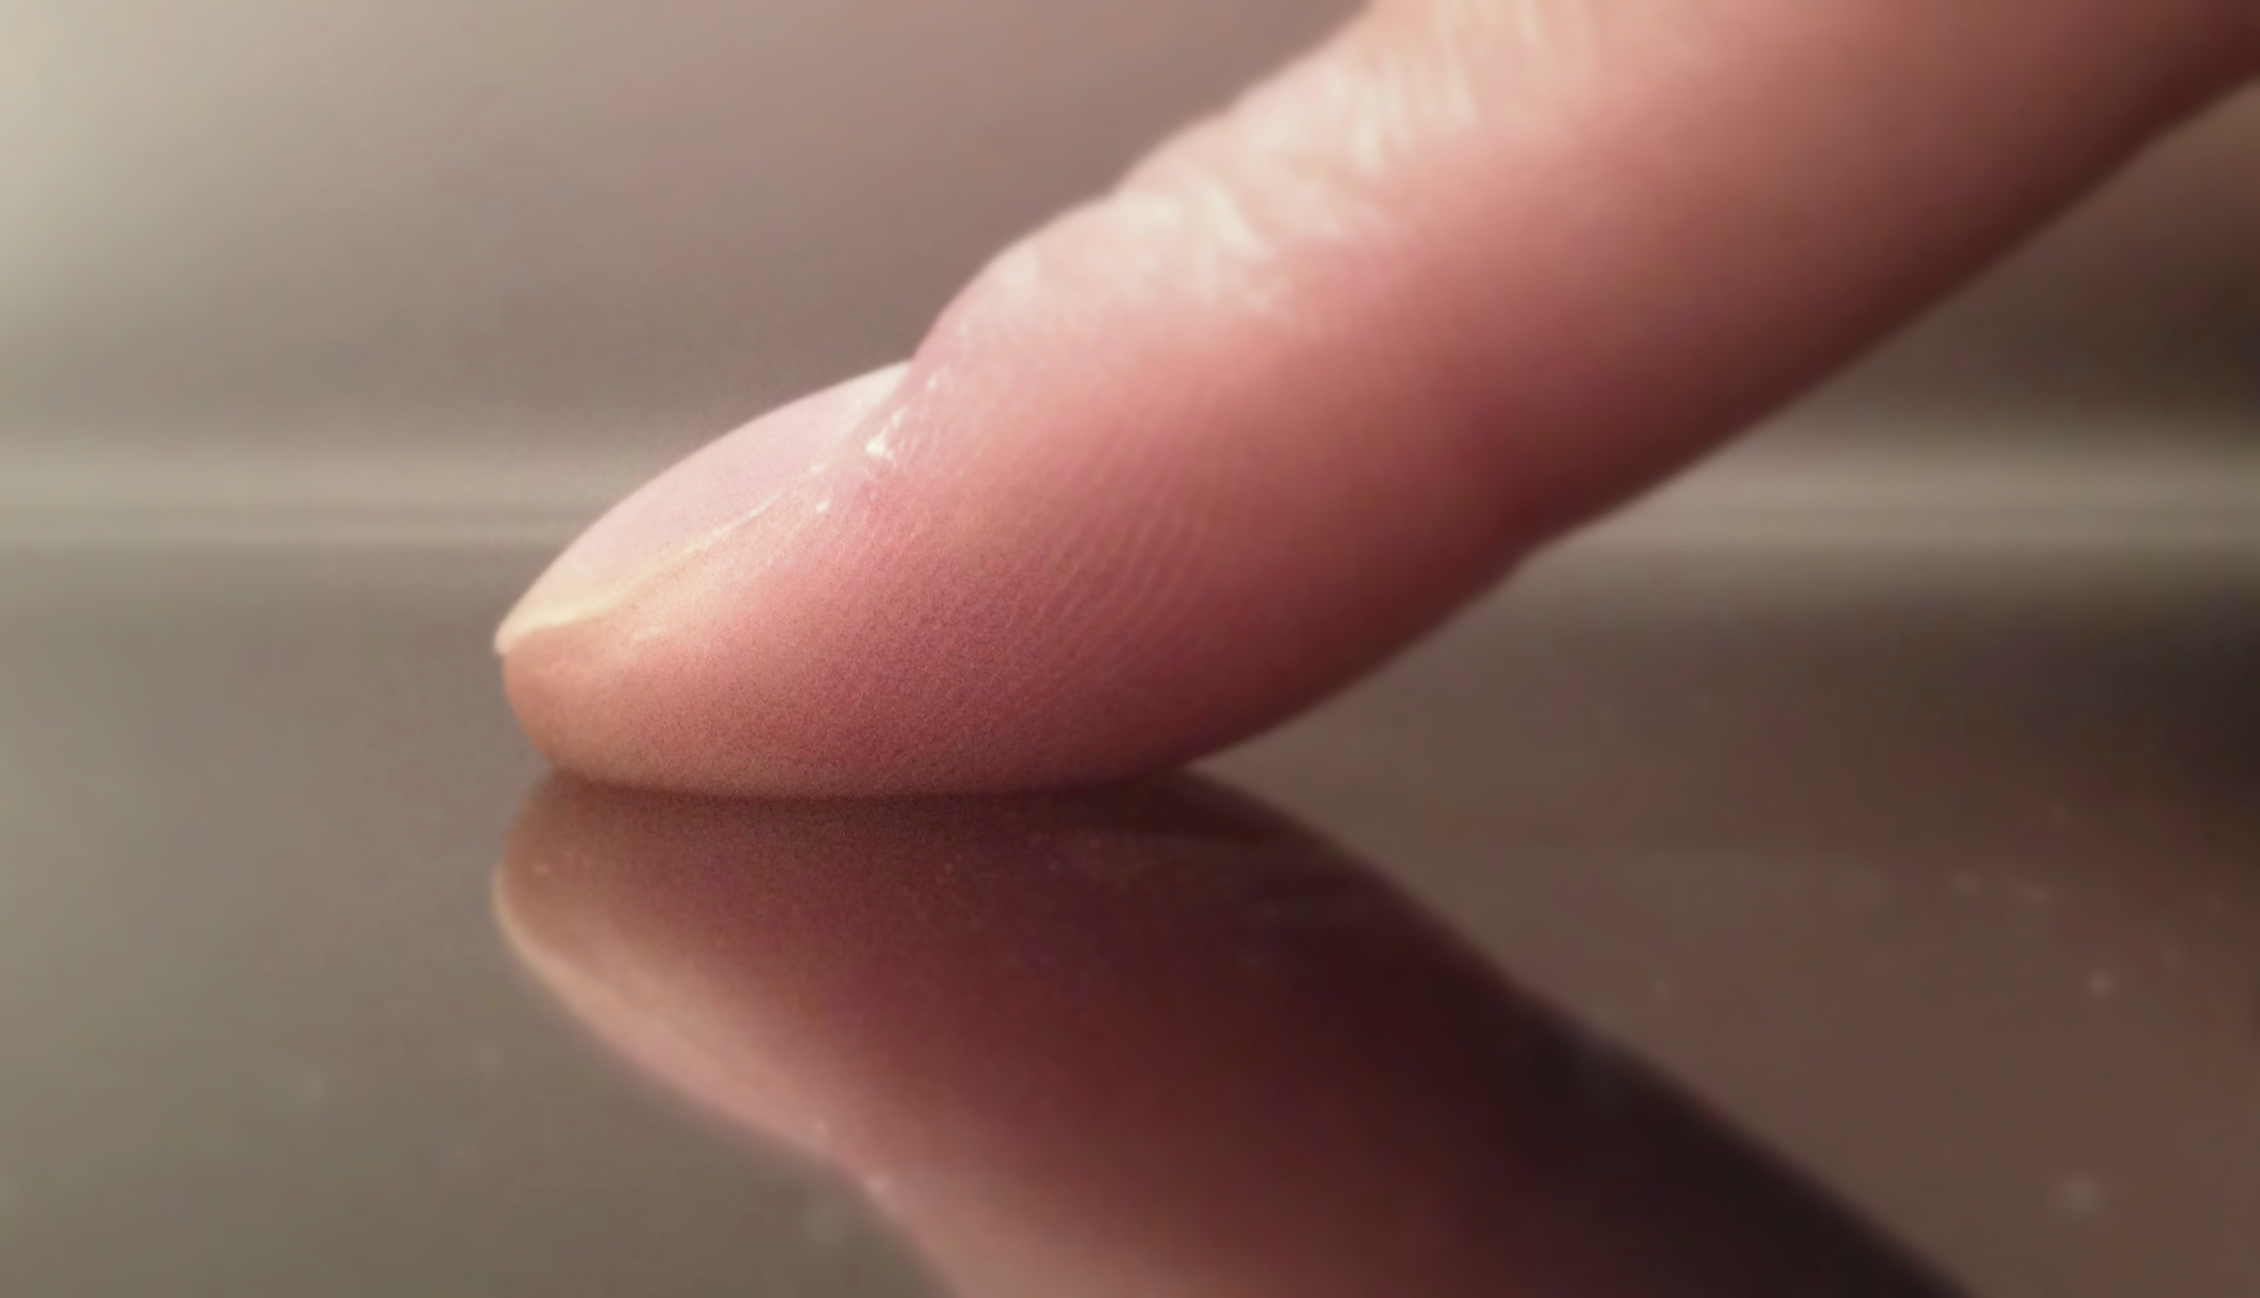
\includegraphics[width=\textwidth]{figures/ffmax}
	\caption{Maximum contact size position}
	\label{fig:ffmax}
\end{subfigure}
\caption{Demonstration of a minimum and a maximum contact size hand position}
\label{fig:ffMinMax}
\end{figure}

%%%%%%%%%%%%%%%%%%%%%%%%%%%%%
%%%%%%%%%%%%%%%%%%%%%%%%%%%%%
%%%%%%%%%%%%%%%%%%%%%%%%%%%%%
%%%%%%%%%%%%%%%%%%%%%%%%%%%%%
%%%%%%%%%%%%%%%%%%%%%%%%%%%%%
%%%%%%%%%%%%%%%%%%%%%%%%%%%%%
\subsection{Assessment}
\label{assessment}


After having completed all the trials, participants instructed to fill a questionnaire to access, rate and finally comment on each of the type of trials they encountered. The questionnaire (Appendix \ref{assessmentFatFinger}) was divided if 4 parts, one for each targeting technique. So, participants had to provide an assessment for all the following type of trials:

 1)\textbf{Feedback \& Discrete Targeting} 2) \textbf{Feedback \& Continuous Targeting} 3) \textbf{No Feedback \& Discrete Targeting} 4) \textbf{No Feedback \& Continuous Targeting}


The assessments had the same structure, and were independent of the type of the trials. Each assessment consists of 6 categories, all on a five point Likert scale. The categories were:


\begin{itemize}
\item \textbf{Smoothness during operation.} The user should rate the smoothness during the operation of the specified Trial type. Smoothness behaves as a general factor that is totally subjective. Signs of roughness can be a slow rate frame in the graphics, or lack on the accuracy of the feedback line. 

\emph{\textbf{Scale}: Very rough (1) - Very smooth (5)}.


\item \textbf{Operation speed.} It can be anything at all. If participants had the feeling the everything flows in a normal rate then the should rate it with 3 which is the normal speed. In this index the best rating is considered 3.

\emph{\textbf{Scale}: Too fast (1) - 2 - Normal (3) - 4 - Too slow (5)}.

\item \textbf{Finger fatigue.} Participants here can record the level of finger fatigue through the corresponding type of trial in this experiment.

\emph{\textbf{Scale}: None (1) - Very high (5)}.

\item \textbf{Wrist fatigue.} Participants here can record the level of wrist fatigue through the corresponding type of trial in experiment.

\emph{\textbf{Scale}: None (1) - Very high (5)}.

\item \textbf{General comfort.} The meaning is inferred from its name. What we ask for, is a general impression on how comfortable this type of trial was. Of course there is interference between this factor and the wrist and finger fatigue ones. However, a type of trial might be comfortable under normal use, but it may cose fatigue in longer use.

\emph{\textbf{Scale}: Very uncomfortable (1) - Very comfortable (5)}.

\item \textbf{Overall assessment.} It measures the general impression of this type. It is measured in usability factors. Thus rating 1 means that it was easy to use and in turn, rating 5 that it was really tough to use it.

\emph{\textbf{Scale}: Very difficult to use (1) - Very easy to use (5)}.
\end{itemize}

Finally, at the bottom of each page there was a comment section, in which participants was asked to comment any advantages or disadvantages they might have encountered during the operation of each type of trial. It was not a required section, however many participants shared their thoughts with us, and we did extracted some really important results out of them.









%%%%%%%%%%%%%%%%%%%%%%%%%%%%%
%%%%%%%%%%%%%%%%%%%%%%%%%%%%%
%%%%%%%%%%%%%%%%%%%%%%%%%%%%%
%%%%%%%%%%%%%%%%%%%%%%%%%%%%%
%%%%%%%%%%%%%%%%%%%%%%%%%%%%%
%%%%%%%%%%%%%%%%%%%%%%%%%%%%%
\section{Participants}

We recruited 26 participants to participate in our study ranging in age from 19 to 52 years old. They had to fill in a Demographic information form from which we collected the following info.

\begin{figure}[H]
\centering
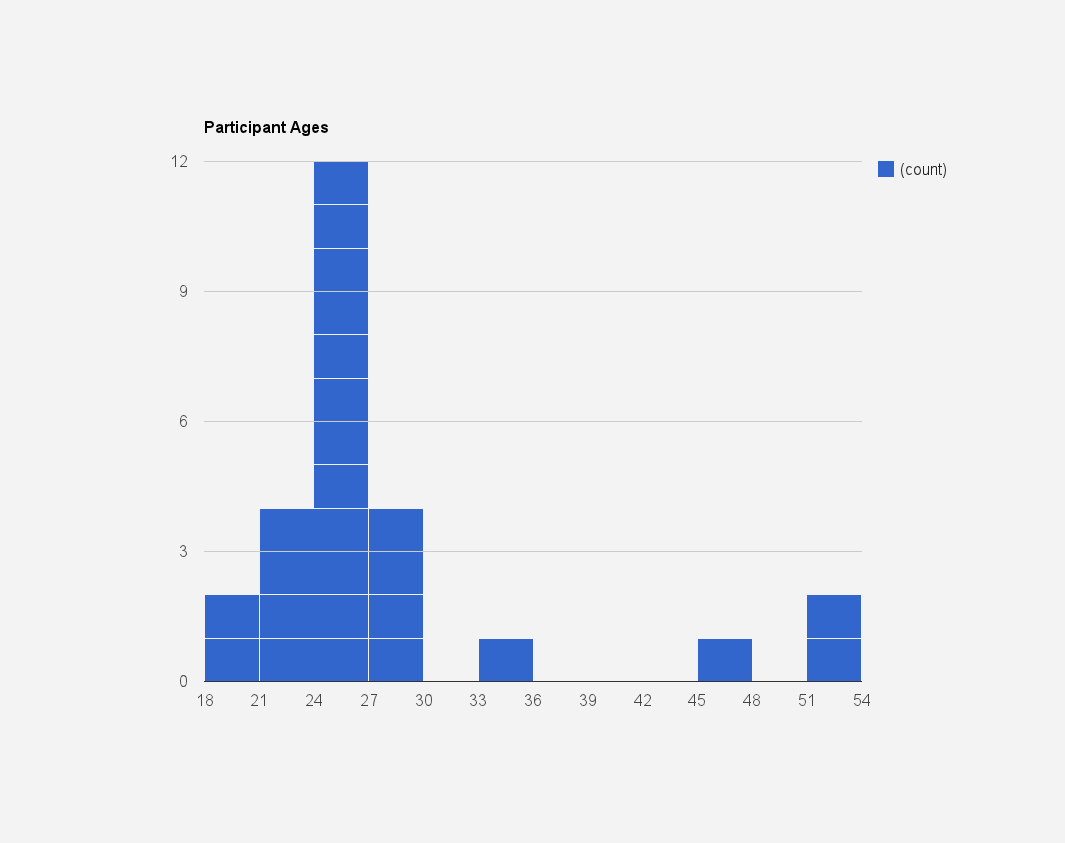
\includegraphics[scale=0.3]{figures/participantAge.png}
\caption{Distribution of participant ages}
\label{fig:participantAge}
\end{figure}

As we can see from Figure \ref{fig:participantAge} participants are mostly ranged between 21 and 30 years old. We also tried to recruit people from older ages, which they might had a different level of experience with tablet devices. therefore we have 2 participants on the 33-48 range and other 2 that are above 50 years old.

\begin{figure}[H]
\centering
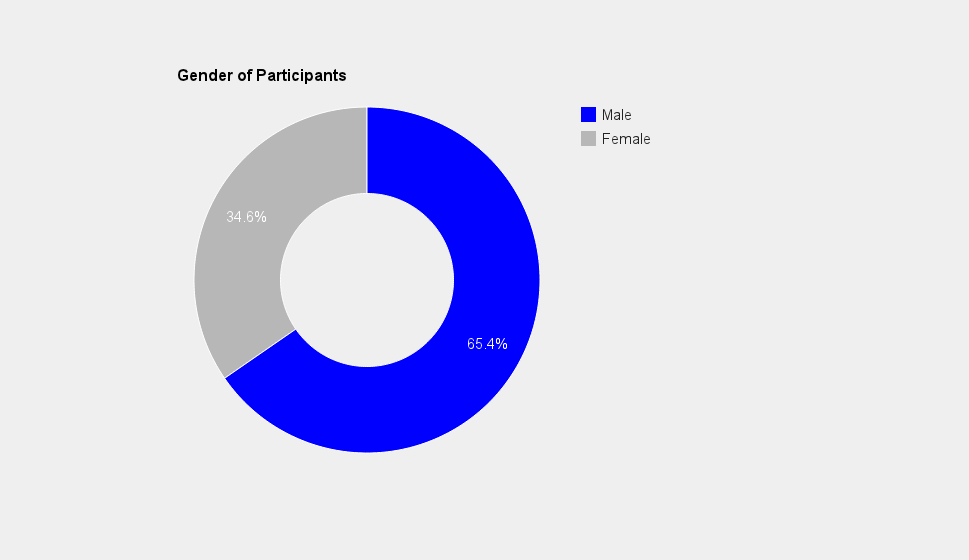
\includegraphics[scale=0.3]{figures/participantGender.png}
\caption{Distribution of participants Gender}
\label{fig:participantGender}
\end{figure}

Participants were mostly male (65.4\%) as it can be observed on Figure \ref{fig:participantGender}. To be precise, we had 17 participants that were male and also 9 more that were female (34.6\%). Also 24 of them were right-handed while only 2 used their left hand for the experiment. Moreover only 21 of them owns a touch based device of any possible kind, and from those just 12 own an actual Tablet device. A mobile, a GPS etc. can be regarded as touch based Devices. We can then conclude that less than half of the users owns a Tablet device, and not specifically an Apple iPad one.

In Figures \ref{fig:experienceTouch}, \ref{fig:experienceTablet} is illustrated how users rated their level of experience on using Touch-Based and Tablet devices respectively.

\begin{figure}[H]
\centering
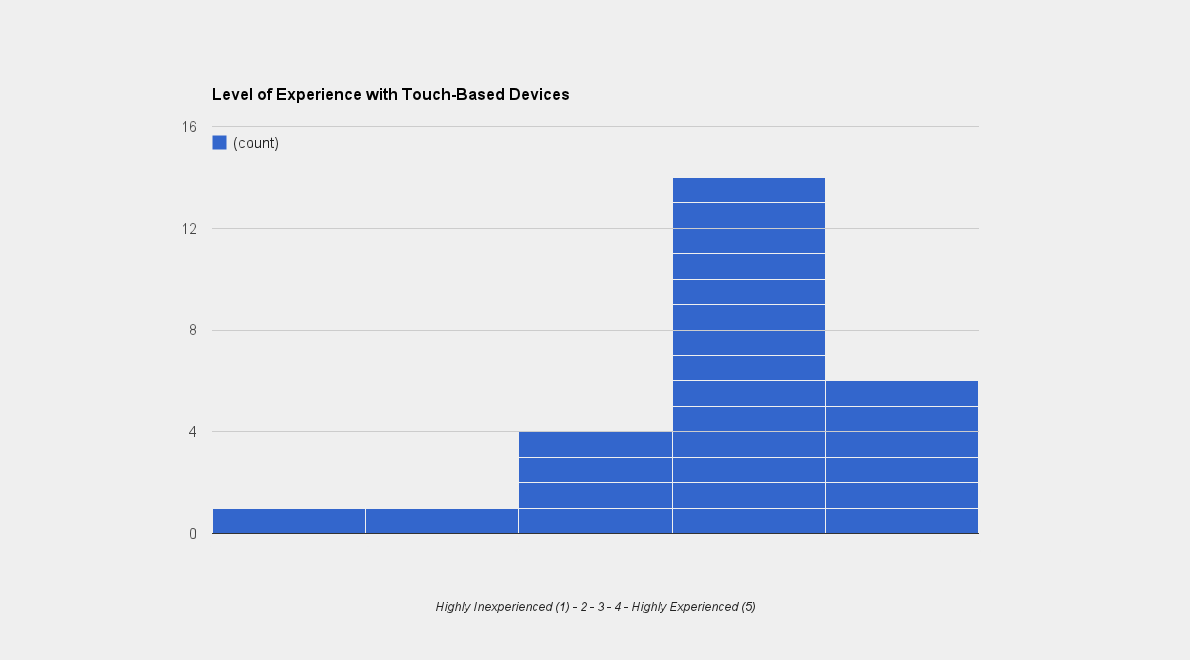
\includegraphics[scale=0.3]{figures/experienceTouch.png}
\caption{Level of Experience with Touch-Based Devices}
\label{fig:experienceTouch}
\end{figure}

\begin{figure}[H]
\centering
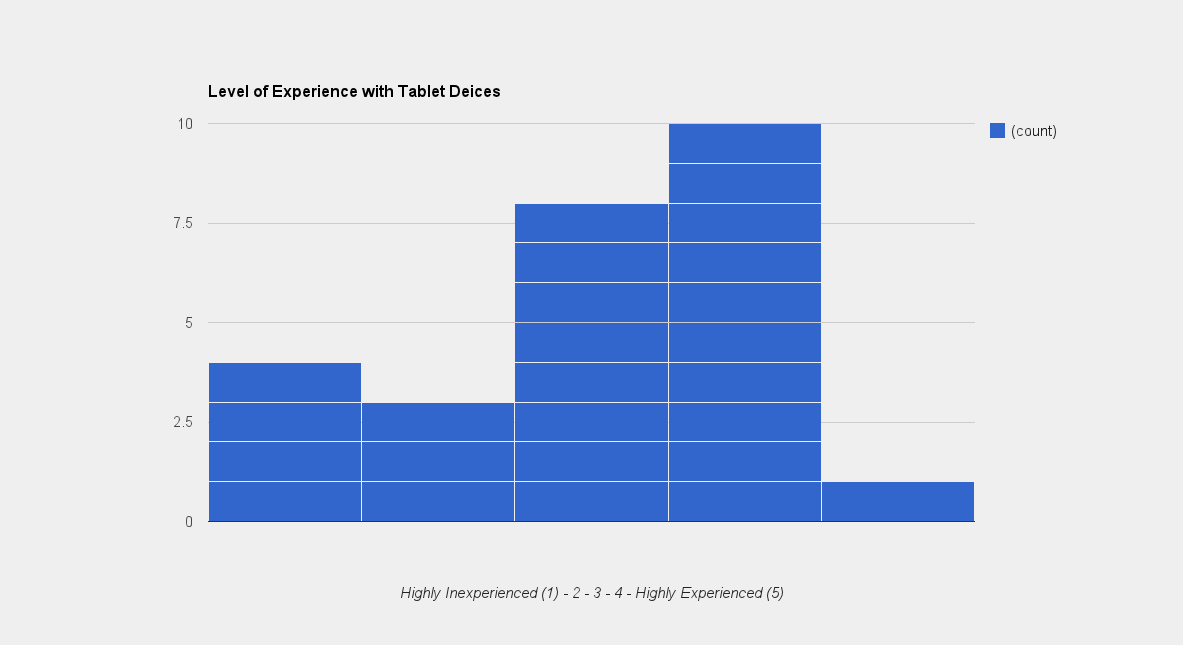
\includegraphics[scale=0.3]{figures/experienceTablet.png}
\caption{Level of Experience with Tablet Devices}
\label{fig:experienceTablet}
\end{figure}

In the above charts, each buckets represents a participant. The more on the right the buckets is (only 5 levels), the more experience this participant has, and vise versa. Thus, we can observe that most of them were experienced using touch-based mobile devices, while fewer were high experienced addressing the tablet devices. This can also be inferred from to the fact that less than half the users owes a tablet device. As a result they have less experience on using one. Finally, it should be mentioned that participants received a small gift, as compensation for their time and effort.




\section{Hypotheses}
\label{sec:hypotheses}

According to and based on our understudying of Fat Finger and on using contact size as the main source for input on tablet devices, we hypothesize the following:

\begin{itemize}
	\item \textbf{\textit{(H1).}} Feedback supplied trials (Discrete or Continuous) outperform No Feedback ones in terms of offset.
	\item \textbf{\textit{(H2).}} No Feedback \& Discrete outperforms No Feedback \& Continuous in terms of offset.
	\item \textbf{\textit{(H3).}} Task completion time will be gradually decreased over time.
	\item \textbf{\textit{(H4).}} Error rates will be gradually decreased over time.
	\item \textbf{\textit{(H5).}} Task competition time, when feedback is provided, is dependent on the number of elements.
	\item \textbf{\textit{(H6).}} Average contact areas will be subconsciously preferred by users, as this is the natural position of the finger.
	\item \textbf{\textit{(H7).}} Feedback \& Discrete is the most preferred type of trial, as it best combines speed and accuracy.
\end{itemize}




